\documentclass[tikz,border=15pt]{standalone}
\usepackage{amsmath,amssymb}
\usetikzlibrary{calc}

\begin{document}
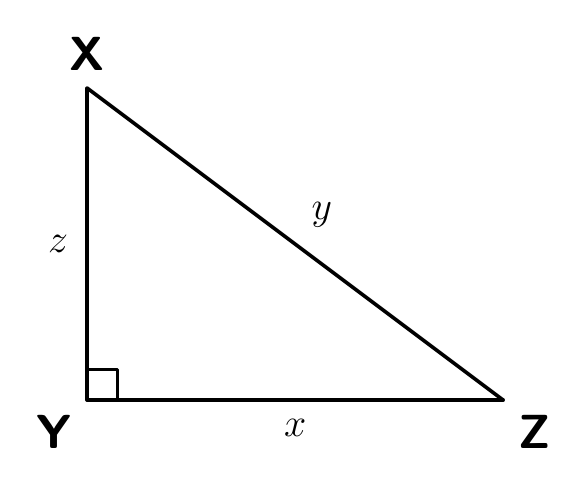
\begin{tikzpicture}[scale=1.1, line cap=round, line join=round]
  % Right triangle XYZ
  \coordinate (Y) at (0, 0);
  \coordinate (X) at (0, 3.6);
  \coordinate (Z) at (4.8, 0);

  % Edges
  \draw[line width=1.3pt] (Y) -- (X) node[midway, left=3pt, font=\Large] {$z$};
  \draw[line width=1.3pt] (Y) -- (Z) node[midway, below=3pt, font=\Large] {$x$};
  \draw[line width=1.3pt] (X) -- (Z) node[midway, above right=2pt, font=\Large] {$y$};

  % Right angle mark at Y
  \draw[line width=1.0pt] (0, 0.35) -- (0.35, 0.35) -- (0.35, 0);

  % Vertex labels
  \node[above=3pt, font=\LARGE\sffamily\bfseries] at (X) {X};
  \node[below left=2pt, font=\LARGE\sffamily\bfseries] at (Y) {Y};
  \node[below right=2pt, font=\LARGE\sffamily\bfseries] at (Z) {Z};

\end{tikzpicture}
\end{document}
